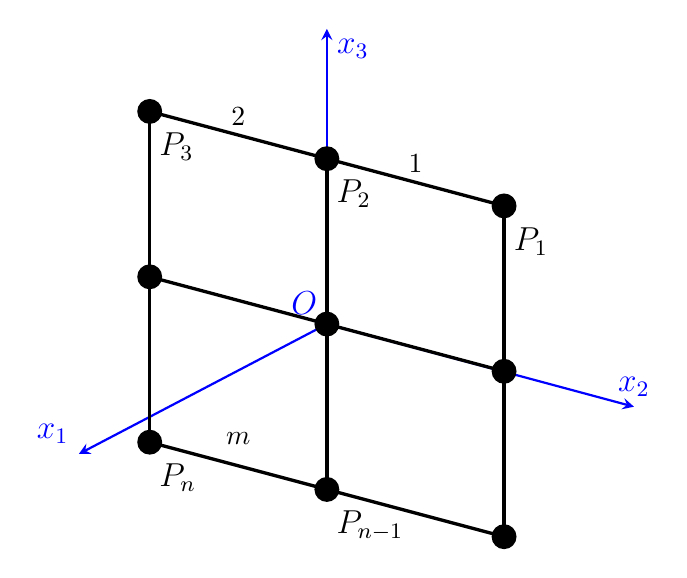
\begin{tikzpicture}[scale=1.5, >=stealth, every node/.style={scale=1.0}]

    % Coordinate dei nodi della griglia (prospettiva isometrica/3D semplificata)
    % Riga superiore
    \coordinate (P3) at (-1.5, 1.8);
    \coordinate (P2) at (0, 1.4);
    \coordinate (P1) at (1.5, 1.0);
    
    % Riga centrale
    \coordinate (M3) at (-1.5, 0.4);
    \coordinate (O)  at (0, 0);
    \coordinate (M1) at (1.5, -0.4);
    
    % Riga inferiore
    \coordinate (Pn)   at (-1.5, -1.0);
    \coordinate (Pn1)  at (0, -1.4);
    \coordinate (B1)   at (1.5, -1.8);

    % --- ASSI CARTESIANI (In blu, posizionati sotto i nodi per non sovrapporsi graficamente) ---
    \draw[blue, thick, ->] (O) -- (-2.1, -1.1) node[above left, font=\large] {$x_1$};
    \draw[blue, thick, ->] (O) -- (2.6, -0.7) node[above, font=\large] {$x_2$};
    \draw[blue, thick, ->] (O) -- (0, 2.5) node[below right, font=\large] {$x_3$};
    
    % Origine degli assi
    \node[blue, above left, font=\large\bfseries] at (O) {$O$};

    % --- LINEE DELLA RETE (Funi) ---
    % Linee orizzontali (corde)
    \draw[very thick, black] (P3) -- (P2) -- (P1);
    \draw[very thick, black] (M3) -- (O) -- (M1);
    \draw[very thick, black] (Pn) -- (Pn1) -- (B1);
    
    % Linee verticali (montanti)
    \draw[very thick, black] (P3) -- (M3) -- (Pn);
    \draw[very thick, black] (P2) -- (O) -- (Pn1);
    \draw[very thick, black] (P1) -- (M1) -- (B1);

    % --- NODI (Cerchi neri) ---
    \foreach \nodo in {P3, P2, P1, M3, O, M1, Pn, Pn1, B1} {
        \fill[black] (\nodo) circle (3.0pt);
    }

    % --- ETICHETTE DEI NODI E DEGLI ELEMENTI ---
    % Nodi superiori
    \node[below right, font=\large] at (-1.5, 1.7) {$P_3$};
    \node[below right, font=\large] at (0, 1.3) {$P_2$};
    \node[below right, font=\large] at (1.5, 0.9) {$P_1$};
    
    % Nodi inferiori
    \node[below right, font=\large] at (-1.5, -1.1) {$P_n$};
    \node[below right, font=\large] at (0, -1.5) {$P_{n-1}$};
    
    % Numerazione elementi (sopra le campate)
    \node[above, font=\normalsize] at (-0.75, 1.6) {$2$};
    \node[above, font=\normalsize] at (0.75, 1.2) {$1$};
    \node[above, font=\normalsize] at (-0.75, -1.1) {$m$};

\end{tikzpicture}